

\documentclass{article}

% Recommended, but optional, packages for figures and better typesetting:
\usepackage{microtype}
\usepackage{graphicx}
\graphicspath{ {./} }
\usepackage{subfigure}
\usepackage{booktabs} % for professional tables
\usepackage{amsmath}

% hyperref makes hyperlinks in the resulting PDF.
% If your build breaks (sometimes temporarily if a hyperlink spans a page)
% please comment out the following usepackage line and replace
% \usepackage{icml2019} with \usepackage[nohyperref]{icml2019} above.
\usepackage{hyperref}

% Attempt to make hyperref and algorithmic work together better:
\newcommand{\theHalgorithm}{\arabic{algorithm}}

% Use the following line for the initial blind version submitted for review:
%\usepackage{icml2020}

% If accepted, instead use the following line for the camera-ready submission:
\usepackage[accepted]{icml2020}

% The \icmltitle you define below is probably too long as a header.
% Therefore, a short form for the running title is supplied here:
\icmltitlerunning{Text-to-image Implementation of Style GAN}

\begin{document}

\twocolumn[
\icmltitle{Milestone Report: Text-to-image Implementation of Style GAN}

% It is OKAY to include author information, even for blind
% submissions: the style file will automatically remove it for you
% unless you've provided the [accepted] option to the icml2019
% package.

% List of affiliations: The first argument should be a (short)
% identifier you will use later to specify author affiliations
% Academic affiliations should list Department, University, City, Region, Country
% Industry affiliations should list Company, City, Region, Country

% You can specify symbols, otherwise they are numbered in order.
% Ideally, you should not use this facility. Affiliations will be numbered
% in order of appearance and this is the preferred way.
\icmlsetsymbol{equal}{*}

\begin{icmlauthorlist}
\icmlauthor{Fei Zheng fz2277}{equal,to}
\icmlauthor{Chirong Zhang cz2533}{equal,to}
\icmlauthor{Xiaoxi Zhao xz2740}{equal,to}
\end{icmlauthorlist}

\icmlaffiliation{to}{Department of Statistics, Columbia University, New York, USA}

% \icmlcorrespondingauthor{}{}

% You may provide any keywords that you
% find helpful for describing your paper; these are used to populate
% the "keywords" metadata in the PDF but will not be shown in the document
\icmlkeywords{Machine Learning, ICML}

\vskip 0.3in
]

% this must go after the closing bracket ] following \twocolumn[ ...

% This command actually creates the footnote in the first column
% listing the affiliations and the copyright notice.
% The command takes one argument, which is text to display at the start of the footnote.
% The \icmlEqualContribution command is standard text for equal contribution.
% Remove it (just {}) if you do not need this facility.


\printAffiliationsAndNotice{}  % leave blank if no need to mention equal contribution
% \printAffiliationsAndNotice{\icmlEqualContribution} % otherwise use the standard text.

\begin{abstract}
In this project, we propose a Style-Based Attentional Generative Adversarial Network (SBA-GAN) that allows unsupervised disentanglement of high-level attributes and an attention-driven refinement for text-to-image generation. Borrowing from StyleGan literature and AttnGan structure, this new generator can synthesize details at different regions of image by paying attentions to relevant parts in the text and by interpolating styles into different resolutions in the image.
\end{abstract}

\section{Introduction}

Text-to-image (T2I) generation is a an important machine learning task and an active research area in both computer vision and natural language processing. It is a fundamental problem in art generation, logo design, interior design and other computer-aided image synthesize. Recent years, significant progress has been made in text-to-image using generative adversarial networks \cite{gan} such as in AttentionGAN \cite{attngan}, MirrorGAN \cite{mirrorgan}, ObjGAN \cite{objgan}, DMGAN \cite{dmgan}. Despite all these impressive results, alignment of generated image with the input text as well as the generation of high-resolution images still remain challenging.

To address this issue, we propose a Style-Based Attentional Generative Adversarial Network (SBA-GAN). Motivated by the Style-Based Generator Architecture for Generative Adversarial Networks (GAN)\cite{stylegan}, which implemented style transfer techniques\cite{styletransferog} in the generative network.  To generate a single image, our generator starts from a learned constant input instead of a latent random variable and it takes the sentence-level and word-level vectors features to put "constraints" on the generated images. The conditional loss is calculated to guarantee the text and image are aligned. Our generator also adjusts the “style” of the image at each convolution layer based on the latent
code, which can directly controlling the strength of image features at different scales. 

We will evaluate our approach by calculating the inception score\cite{inception} of generated images and the R-precision score\cite{attngan} to check if the images and texts are aligned.

\section{Related work}

Based on the DCGAN\cite{dcgan}, Reed\yrcite{text2image} has proposed an architecture to do text-to-image translation. In his algorithm GAN-CLS\cite{text2image}, he introduces a third type of input consisting of real images with mismatched text in discriminator in addition to the real/fake inputs. This provides an additional signal to the generator. Also, he explores the disentangling of style and content by inverting the generator for style and it turns out captions alone are not informative for style prediction.

AttnGAN \cite{attngan} first came up with the idea to synthesize fine-grained details at different subregions of the image by paying attention to the relevant words in the natual language desciption. MirrorGAN\cite{mirrorgan} borrow the idea of circleGAN\cite{cyclegan} and generate image from text and text back from image.

With the appearance of StyleGAN\cite{stylegan}, researchers have proposed new network structure using it and have observed a great increse in FID score\cite{fid}. LOGAN \cite{logan} which proposes a conditional GAN structure with StyleGAN implemented, has successfully generate conditional logos with high FID. But the paper did not discuss the alignment between the image and the logo label and indeed, some generated logos do not seem to be properly generated conditioned on the given label. Our model, tries to address this problem and introduce the similarity measure between text and the generated images.


\begin{figure*}[htbp]

\centering
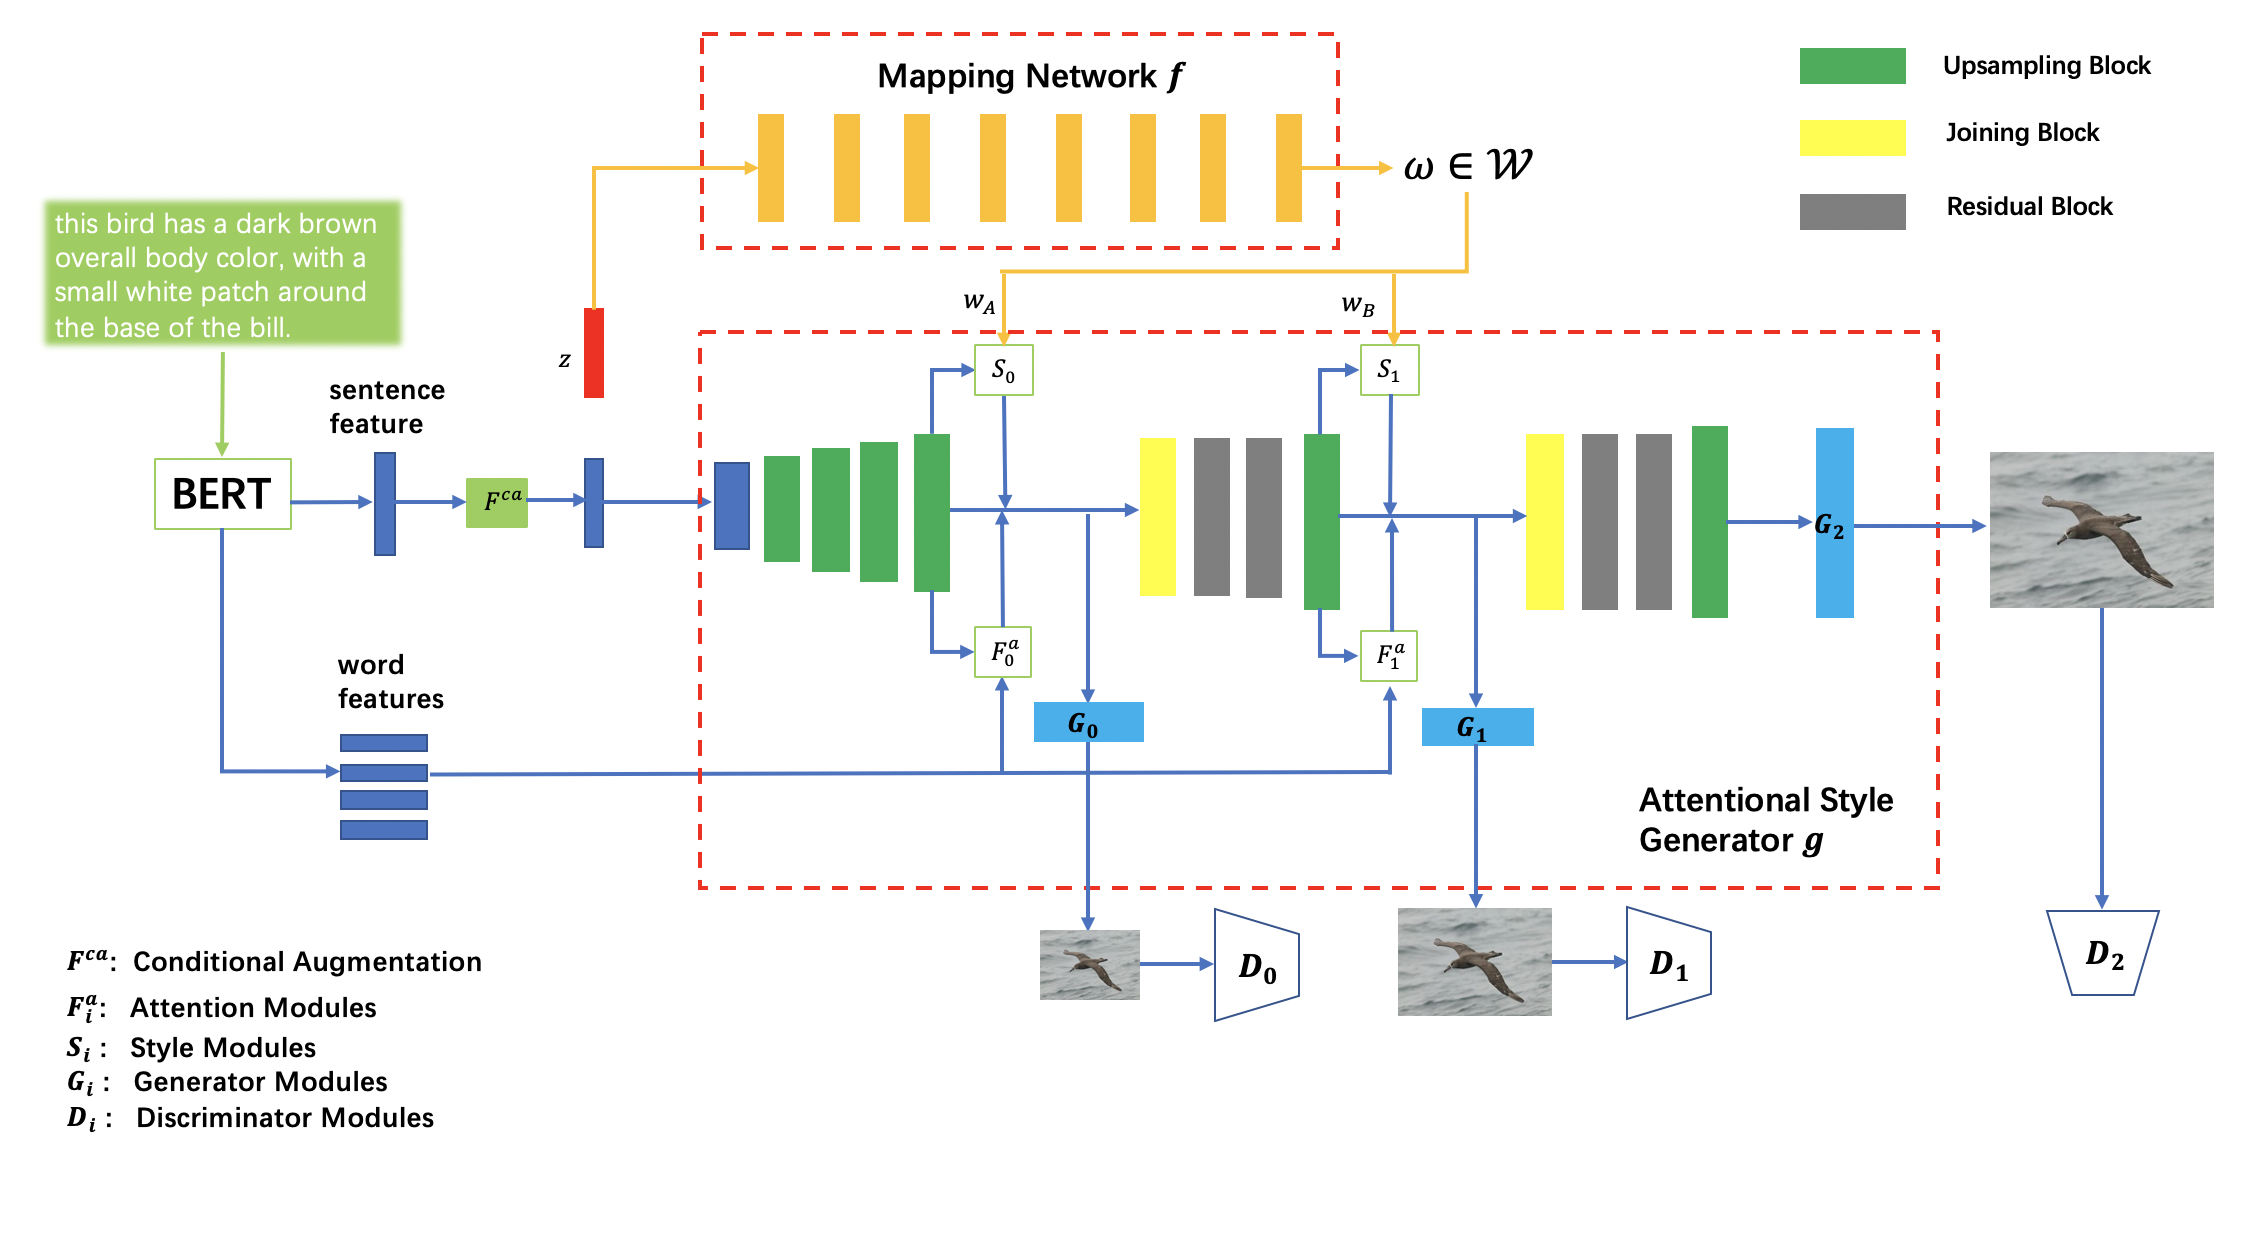
\includegraphics[width=450pt, height=200pt]{milestone/network.png} 
\caption{The architecture of SBA-GAN. The random latent variable is concatenated with conditionally augmented(CA) sentence feature and then goes through the mapping network to an intermediate latent space $\mathcal{W}$. During each step of progressive training process, word features and past images are combined to generate new attentional styles, which are applied later in adaptive instanve normalization(AdaIN) layers. The attentional style generator network $g$ consist of 10 layers -- two for each resolution($4^2 - 256^2$). The discriminator is similar to progressive GAN\cite{progan}.}
\label{model}
\end{figure*}

\section{Style-Based Attentional Generative Adversarial Network}
As shown in Figure \ref{model}, SBA-GAN integrates both StyleGAN\cite{stylegan} and AttnGAN\cite{attngan} and embodies the attention modules into the progressive generation process. Disentangled by mapping network, latent code $w$ can control the style of generated images better. By attention modules, text can influence the objects generation better. Technically, SBA-GAN is mainly consist of two modules: text encoder module, attentional style generator module. We will introduce these modules below.


\subsection{Text Encoder Module}
First, we introduce the text encoder module that transforms the texts to features. BERT\cite{bert} is a great breakthrough in the domain of pre-trained natural language processing. We borrow the pre-trained model and embed the given text description into both word-level features that work mainly in attention modules and sentence-level features that work mainly in generation process. In consideration of limited computation resources, we freeze all the layers in BERT.

Due to the diversity of the text domain and in order to enhance the model robustness, we introduce some noises in sentence-level features by using Conditional Augmentation\cite{stackgan}. In Figure \ref{model}, we use $F^{ca}$ to represent this module.
\begin{equation}
    \bar{e}_{ca} = F^{ca}(\bar{e}),
\end{equation}
where $\bar{e} \in \mathcal{R}^{D}$, $\bar{e}_{ca} \in \mathcal{R}^{D'}$, $D$ is the dimension of embedding features and $D'$ is the dimension after augmentation.

Then we concatenate the augmented sentence embedding with random latent code $z \sim N(0,1)$, which is the input of the generator.

\subsection{Attentional Style Generator Module}
Next we introduce the style-base attentional generator module. We adopt the general structure described in StyleGAN\cite{stylegan}. In the mapping network part, we use a 8-layer MLP to disentangle the latent code $z$ into latent code $w$.
\begin{equation}
    w = MLP(z)
\end{equation}
In the generation part, we follow the practice of StyleGAN and use the structure of ProgressiveGAN\cite{progan} to generate images from resolution $4^2$ to $256^2$ step by step. During each step, we mix the information from both previous image feature $f$ and word-level features $w$ by attention module, which is proposed by AttnGAN\cite{attngan}.
\begin{equation}
    Att = FC(\sum_{l=0}^{L-1} (Uw^l)(softmax(f^T (Uw^l)))^T),
\end{equation}
where $Att \in \mathcal{R}^{T}$, $T$ is the dimension of attetion vector and $U \in \mathcal{R}^{M \times D}$ is to transform the words to the space with same dimension as image. Full connected layer $FC$ is aimed to transform the re-weighted image feature into the space with same dimension as attention vector.

Then we concatenate the attention code with disentangled latent code $w$ and use a learnable affine transformations, which is denote by $A$ in Figure \ref{model}, to specialize it to \textit{styles} $y = (y_s, y_b)$ to control the adaptive instance normalization(AdaIN) operation after each convolution layer of the generation network. The AdaIN operation is defined as:
\begin{equation}
    AdaIN(x_i, y) = y_{s,i} \frac{x_i - \mu(x_i)}{\sigma(x_i)} + y_{b,i},
\end{equation}
where each feature map $x_i$ is normalized separately, and then scaled and biased using the corresponding scalar components from \textit{style} $y$. So the dimension of $y$ is twice the number of features on that layer.

For Discriminator part. We follow the practice of ProgressiveGAN\cite{progan} and reverse generator network except attetion module to attain image features.

\subsection{Objective functions}
Following common practice, we employ the GAN loss that embodies both conditional and unconditional. The loss is defined as
\begin{align}
    \mathcal{L}_{G'} = -\frac{1}{2}\mathrm{E}_{\hat{x} \sim P_G [log(D(\hat{x})]} - \frac{1}{2}\mathrm{E}_{\hat{x} \sim P_G [log(D(\hat{x}, \bar{e})]}
\end{align}
\begin{align}
    \mathcal{L}_{D} = &-\frac{1}{2}\mathrm{E}_{\hat{x} \sim P_{data} [log(D(\hat{x})]} - \frac{1}{2}\mathrm{E}_{\hat{x} \sim P_G [log(1 - D(\hat{x})]} \nonumber \\
    &- \frac{1}{2} \mathrm{E}_{\hat{x} \sim P_{data} [log(D(\hat{x}, \bar{e})]} - \frac{1}{2}\mathrm{E}_{\hat{x} \sim P_G [log(1 - D(\hat{x}, \bar{e})]},
\end{align}
where $x$ is from the true image distribution $P_{data}$ and $\hat{x}$ is from the model distribution $P_G$. The unconditional loss determines whether the image is real or fake and the conditional loss determines whether the image matches the sentence or not.

Apart from the common GAN loss, we also include the cosine similarity score in generation part since this can make generated image and text match better. For text encoder part, we use BERT to attain sentence embedding $\bar{e}$, as described above. For image encoder, we adopt Inception v3\cite{inception} to attain image embedding $\bar{c}$. The cosine similarity score can be calculated as $R(\bar{c}, \bar{e}) = (\bar{c}^T \bar{e})/(\Vert \bar{c} \Vert \Vert \bar{e}\Vert)$.



\section{Experiment}
\subsection{Experiment Setup}
\subsubsection{Dataset}
Same as previous text-to-image methods\cite{attngan,mirrorgan}, our method is evaluated on CUB \cite{WahCUB_200_2011} and COCO\cite{coco} datasets.

CUB dataset consists of 11788 images of 200 categories of birds with about 10 sentences to describe each image. 
and COCO\cite{coco} datasets. COCO dataset is a larger dataset with 123,287 images and 886,284 instances.

\subsubsection{Evaluation Criteria}

We will evaluate our approach by calculating the inception score\cite{inception} of generated images and the R-precision score proposed in AttnGAN \cite{attngan} to check if the images and texts are aligned.
Inception score is a quantitative evaluation measure to the objectiveness and diversity of generated images but cannot reflect whether the generated image is well conditioned on the given text description. 

R-precision is on the other hand, an evaluation metric to measure the similarity of images and the corresponding texts. We calculate the cosine similarities between the image feature and the text feature and count the average accuracy at the different settings: top-r. If the ground truth falls into the top-r candidates, then the image and text are considered aligned, otherwise not.

\subsubsection{Implementation Details}
\subsection{Main Results}
The coding part can be found on github \href{https://github.com/zhengfei0908/SBA-GAN}{https://github.com/zhengfei0908/SBA-GAN}.

The preliminary results can be found on \href{https://drive.google.com/drive/u/1/folders/11J_XfP8IE53kUUfCL9ZGYbF5ZRvPyejj}{https://drive.google.com/drive/u/1/folders/11J_XfP8IE53kUUfCL9ZGYbF5ZRvPyejj}

We haven't finished running our model so we don't have any generated images for now, but we will upload our generated images by Sunday night.

\newpage

% In the unusual situation where you want a paper to appear in the
% references without citing it in the main text, use \nocite
\nocite{langley00}

\bibliography{example_paper}
\bibliographystyle{icml2020}


%%%%%%%%%%%%%%%%%%%%%%%%%%%%%%%%%%%%%%%%%%%%%%%%%%%%%%%%%%%%%%%%%%%%%%%%%%%%%%%
%%%%%%%%%%%%%%%%%%%%%%%%%%%%%%%%%%%%%%%%%%%%%%%%%%%%%%%%%%%%%%%%%%%%%%%%%%%%%%%
% DELETE THIS PART. DO NOT PLACE CONTENT AFTER THE REFERENCES!
%%%%%%%%%%%%%%%%%%%%%%%%%%%%%%%%%%%%%%%%%%%%%%%%%%%%%%%%%%%%%%%%%%%%%%%%%%%%%%%
%%%%%%%%%%%%%%%%%%%%%%%%%%%%%%%%%%%%%%%%%%%%%%%%%%%%%%%%%%%%%%%%%%%%%%%%%%%%%%%
% \appendix
% \section{Do \emph{not} have an appendix here}

% \textbf{\emph{Do not put content after the references.}}
% %
% Put anything that you might normally include after the references in a separate
% supplementary file.

% We recommend that you build supplementary material in a separate document.
% If you must create one PDF and cut it up, please be careful to use a tool that
% doesn't alter the margins, and that doesn't aggressively rewrite the PDF file.
% pdftk usually works fine. 

% \textbf{Please do not use Apple's preview to cut off supplementary material.} In
% previous years it has altered margins, and created headaches at the camera-ready
% stage. 
%%%%%%%%%%%%%%%%%%%%%%%%%%%%%%%%%%%%%%%%%%%%%%%%%%%%%%%%%%%%%%%%%%%%%%%%%%%%%%%
%%%%%%%%%%%%%%%%%%%%%%%%%%%%%%%%%%%%%%%%%%%%%%%%%%%%%%%%%%%%%%%%%%%%%%%%%%%%%%%


\end{document}


% This document was modified from the file originally made available by
% Pat Langley and Andrea Danyluk for ICML-2K. This version was created
% by Iain Murray in 2018, and modified by Alexandre Bouchard in
% 2019. Previous contributors include Dan Roy, Lise Getoor and Tobias
% Scheffer, which was slightly modified from the 2010 version by
% Thorsten Joachims & Johannes Fuernkranz, slightly modified from the
% 2009 version by Kiri Wagstaff and Sam Roweis's 2008 version, which is
% slightly modified from Prasad Tadepalli's 2007 version which is a
% lightly changed version of the previous year's version by Andrew
% Moore, which was in turn edited from those of Kristian Kersting and
% Codrina Lauth. Alex Smola contributed to the algorithmic style files.
